\documentclass[10pt, a4paper]{article}
\usepackage[utf8]{inputenc}
\usepackage[spanish]{babel}
\usepackage[margin=1.5cm]{geometry}
\usepackage{graphicx}
\usepackage{booktabs} 
\usepackage{pgfplots} 
\pgfplotsset{compat=1.18}
\usepackage{hyperref}
\hypersetup{
	colorlinks=true,
	linkbordercolor=white,
	citecolor=black,
	linkcolor=black
}
\usepackage{cleveref}
\usepackage{enumitem}
\usepackage{etoolbox}
\usepackage{authblk}
\usepackage{xcolor}
\usepackage{float}

\makeatletter
\apptocmd{\@floatboxreset}{\centering}{}{}
\makeatother

\title{\Large \textbf{Proyecto Sistemas Distribuidos}}
\author[1]{Solon Losada Cadena}
\author[1]{Juan Pablo Peña Bernal}
\author[1]{Alejandro González Ochoa}
\affil[1]{Departamento de Ingeniería de Sistemas, Pontificia Universidad Javeriana, Bogotá, 110231, Colombia.}
\date{}

\begin{document}
	
	\maketitle
	\vspace{-1.2cm}
	
	\begin{center}
		\small Autores: \href{mailto:solon.losadac@javeriana.edu.co}{\color{blue}solon.losadac@javeriana.edu.co}; \href{mailto:jp.penab@javeriana.edu.co}{\color{blue}jp.penab@javeriana.edu.co}; \href{mailto:alejandro.gonzalez.o1055@javeriana.edu.co}{\color{blue}alejandro.gonzalez.o1055@javeriana.edu.co}
	\end{center}
	
	
	\begin{center}
		\textbf{Docente:} Ricardo Hjalmar González García \\
		\textbf{Fecha:} 8 de octubre de 2026
	\end{center}
	
	\vspace{0.7cm}
	
	
	% ---------------------------------------------------------
	% PRIMERA ENTREGA (Max 5 pages)
	% ---------------------------------------------------------
	
	
	{\small \textbf{\textit{Keywords}---}proceso de Reserva Modificación y Consulta, ZeroMQ, Sistema de Reserva de Boletos.\par}
	
	
	\section{Modelos del sistema}
	\label{sec:models}
	
	
	A continuación se explican los modelos que usa el sistema de reservas.
	
	\subsection{Modelo Arquitectónico}
	\label{sec:models_arch}
	
	De acuerdo con la arquitectura del software que se nos dio a diseñar e implementar, observamos un \textbf{estilo arquitectónico de capas}: (\cref{fig:layers_model}).
	
	\begin{figure}[H]
		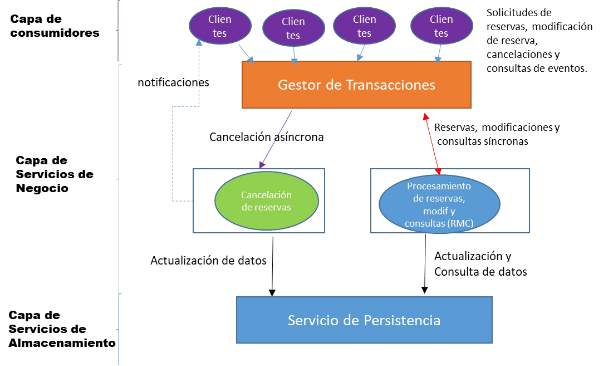
\includegraphics[width=0.7\textwidth]{Images/Modelo de capas sistema.png}
		\caption{Modelo arquitectónico de 3 capas del sistema}
		\label{fig:layers_model}
	\end{figure}
	
	La \textbf{capa de consumidores} envía al gestor de transacciones las solicitudes de los clientes: reserva, modificación, consulta y cancelación. También recibe la notificación que confirma cuándo una cancelación se hizo efectiva.
	
	La \textbf{capa de servicios} tiene tres procesos. El \textit{gestor de transacciones} (GT) enruta cada petición por uno de dos canales. El canal síncrono lleva las reservas, modificaciones y consultas al servicio RMC: el cliente se conecta al GT con REQ/ROUTER y el GT reparte el trabajo al RMC con ROUTER/DEALER. El canal asíncrono lleva las cancelaciones al \textit{servicio de cancelación y notificación} mediante PUSH/PULL; una vez liberados los puestos, ese servicio notifica directamente al cliente.
	
	Finalmente, la \textbf{capa de almacenamiento} garantiza la persistencia de las reservas de todo el sistema. El servicio de persistencia es el único que accede a la base de datos PostgreSQL, con operaciones CRUD, y recibe las peticiones del RMC y del servicio de cancelación mediante REQ/ROUTER.
	
	
	\subsection{Modelo de Interacción}
	\label{sec:models_exch}
	
	En este proyecto se combinan los modelos de interacción síncrono y asíncrono.
	El modelo síncrono se usa en las reservas, modificaciones y consultas. El gestor de transacciones recibe la solicitud y la enruta al servicio RMC, que pide el resultado a la capa de almacenamiento. El cliente no recibe respuesta hasta que termina todo ese recorrido. Entre el cliente y el gestor se usa el patrón \textbf{request-router}, porque permite atender varias solicitudes al mismo tiempo: los clientes son el \textit{request}, el gestor es el \textit{router} y cada solicitud lleva un identificador único para que la respuesta llegue a quien la hizo. Entre el gestor y el RMC se usa ROUTER/DEALER, y entre el RMC y persistencia, REQ/ROUTER.
	El modelo asíncrono se usa en las cancelaciones. El gestor acepta la cancelación y responde de inmediato al cliente con una confirmación de recepción; el servicio de cancelación hace el trabajo después. Cuando persistencia confirma que los puestos quedaron liberados, ese servicio notifica al cliente en la dirección que este incluyó en su solicitud. El trabajo pasa del gestor al servicio de cancelación por PUSH/PULL (pipeline), porque reparte las tareas por turnos entre varios consumidores y eso facilita escalar más adelante.
	
	\subsection{Modelo de Fallos}
	\label{sec:models_fail}
	Se espera que el gestor de transacciones o el RMC (servicio que procesa reservas, modificaciones y consultas) puedan fallar. Por eso se plantea un fallo de tipo \textit{fail-stop}: el proceso se detiene y los demás pueden detectarlo. Esto es grave porque la falla debe ser transparente para los clientes, y tanto el gestor como el RMC concentran funciones críticas. En el peor caso uno de los dos sufre un \textit{crash}; la propuesta para tolerarlo está en la sección~\ref{sec:scalability}.
	
	
	
	\subsection{Modelo de Seguridad}
	\label{sec:models_secu}
	Si el canal ZeroMQ no se asegura, los mensajes viajan en texto plano y un atacante puede interceptarlos, así que la confidencialidad y la integridad quedan expuestas. La disponibilidad también puede verse afectada: un ataque de denegación de servicio (DoS) contra el gestor de transacciones podría saturarlo.
	
	
	\section{Diseño del Sistema}
	\label{sec:base_arch}
	
	El diseño se documenta con cuatro diagramas: componentes, despliegue y clases (vistas estáticas de la estructura lógica y física del SRB) y secuencia (vista dinámica de su comportamiento).
	
	\subsection{Diagrama de Componentes}
	\begin{figure}[H]
		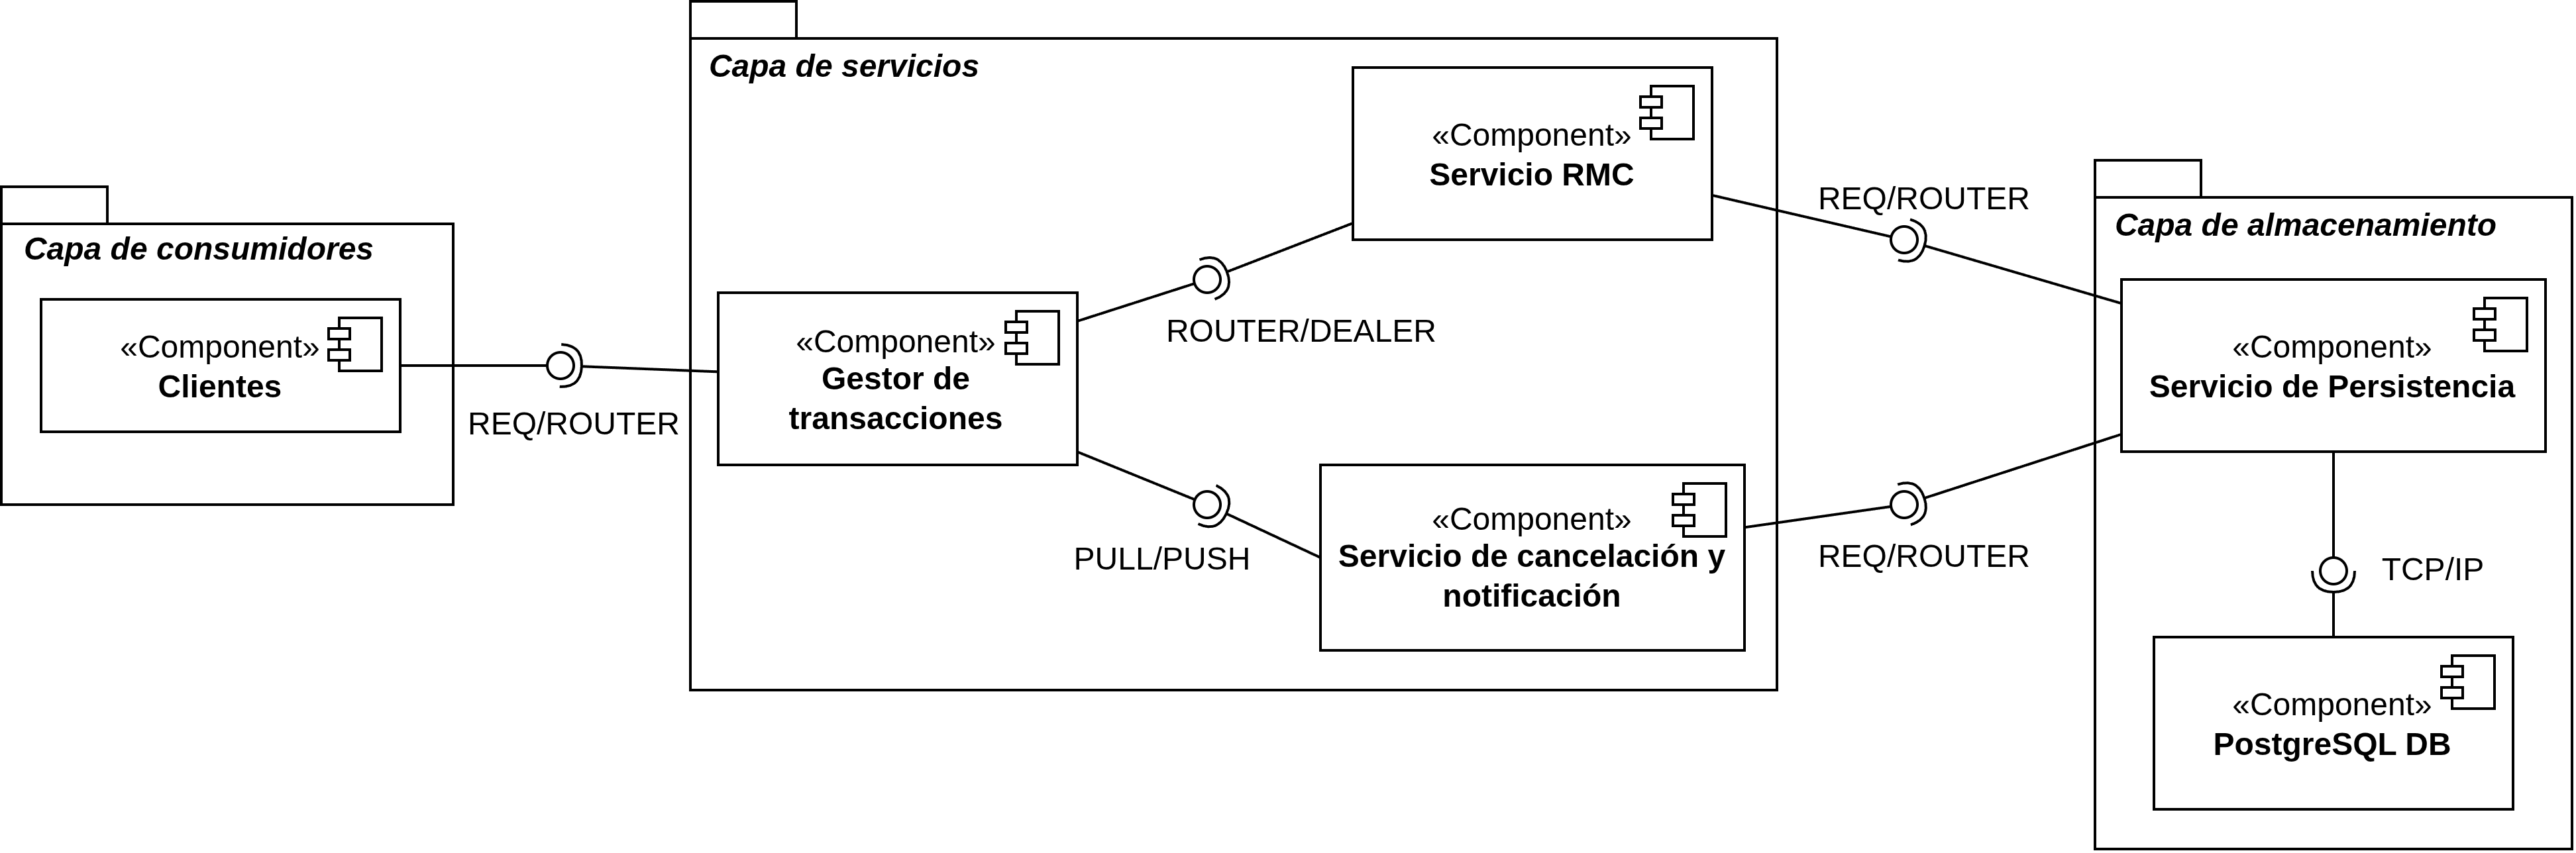
\includegraphics[width=1\textwidth]{Images/Diagrama de Componentes.png}
		\caption{Diagrama de componentes del SRB}
		\label{fig:comp_diagram}
	\end{figure}
	El diagrama muestra cómo se relacionan los componentes y qué protocolo usa cada conexión.
	Los clientes se comunican con el gestor mediante REQ/ROUTER, y el gestor con el RMC mediante ROUTER/DEALER. El RMC y el servicio de cancelación se conectan a persistencia con REQ/ROUTER. Las cancelaciones viajan por PUSH/PULL, un pipeline asíncrono, y el servicio de cancelación devuelve la notificación al cliente por una conexión directa.
	El servicio de persistencia es el único componente que accede a PostgreSQL, por TCP/IP. Recibe las solicitudes del RMC y del servicio de cancelación.
	
	\subsection{Diagrama de Despliegue}
	
	\begin{figure}[H]
		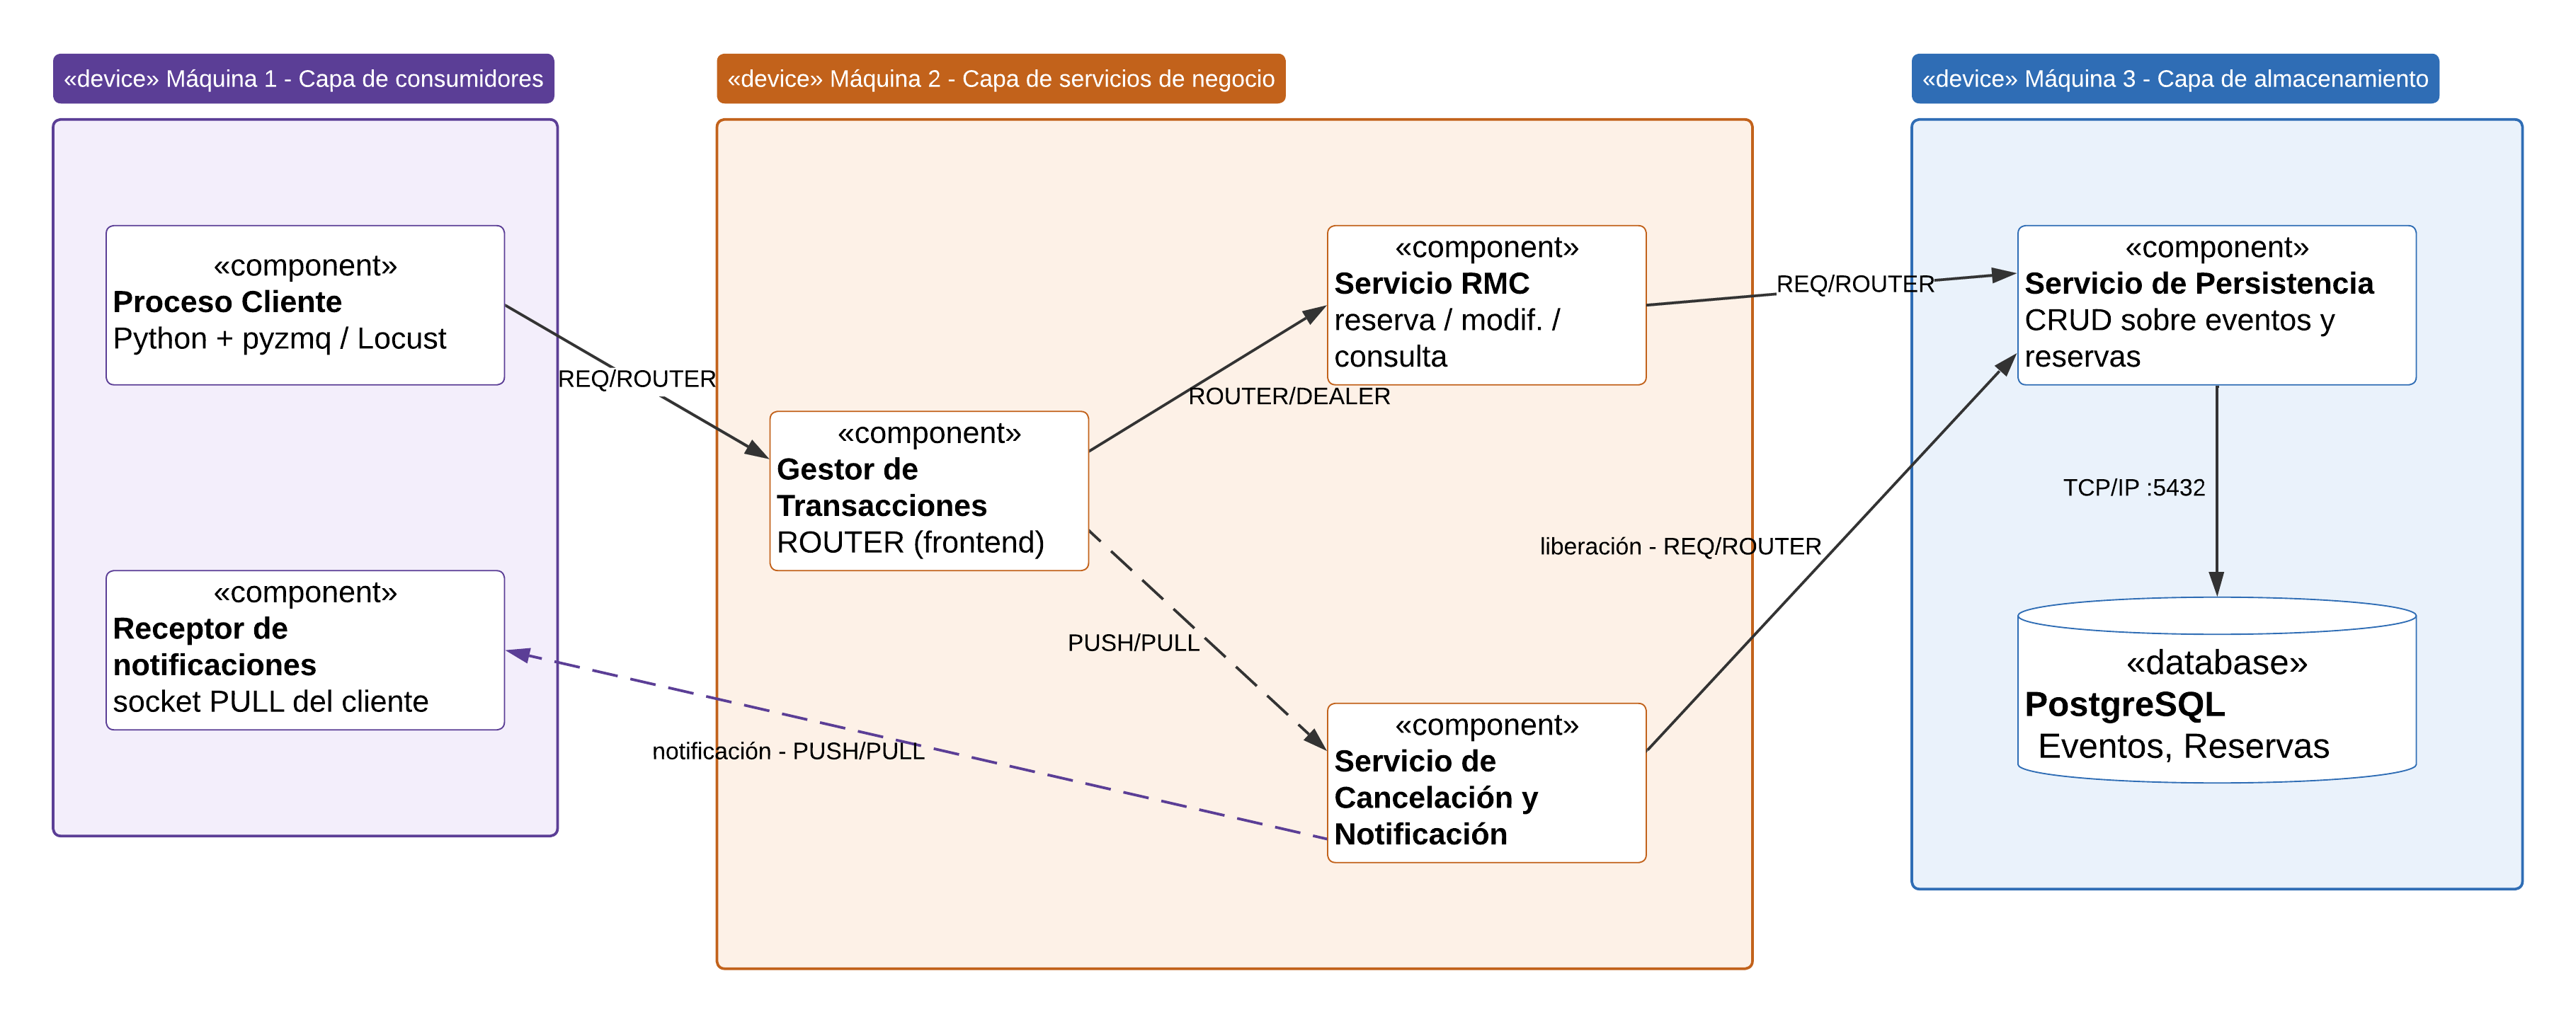
\includegraphics[width=1\textwidth]{Images/Diagrama de Despliegue.png}
		\caption{Diagrama de Despliegue del SRB}
		\label{fig:deploy_diagram}
	\end{figure}
	La figura~\ref{fig:deploy_diagram} muestra la distribución del sistema en tres máquinas, una por capa. En la primera se ejecutan los clientes, desarrollados en Python con pyzmq, y el generador de carga. Cada cliente cuenta además con un receptor PULL para recibir el resultado de sus cancelaciones.

    En la segunda máquina se ubican el Gestor de Transacciones, el servicio RMC y el servicio de Cancelación y Notificación. El gestor recibe las solicitudes y selecciona su destino: las consultas, reservas y modificaciones pasan al RMC, mientras que las cancelaciones se envían por PUSH/PULL para procesarlas sin mantener al cliente esperando el resultado final. La figura representa ROUTER/DEALER en la comunicación entre el gestor y el RMC.

    La tercera máquina contiene el servicio de persistencia y PostgreSQL, que corre en un contenedor Docker (primario en el puerto 5432 y réplica en streaming de solo lectura en el 5433, ambos accesibles solo desde esa máquina). Junto a las bases corre pgAdmin, que permite ver su contenido en un entorno gráfico. El RMC y el servicio de cancelación piden los cambios a persistencia; los clientes no acceden a la base. La notificación final llega desde el servicio de cancelación al receptor del cliente, en la dirección que este proporcionó.
	
	\subsection{Diagrama de Clases}
	
	\begin{figure}[H]
		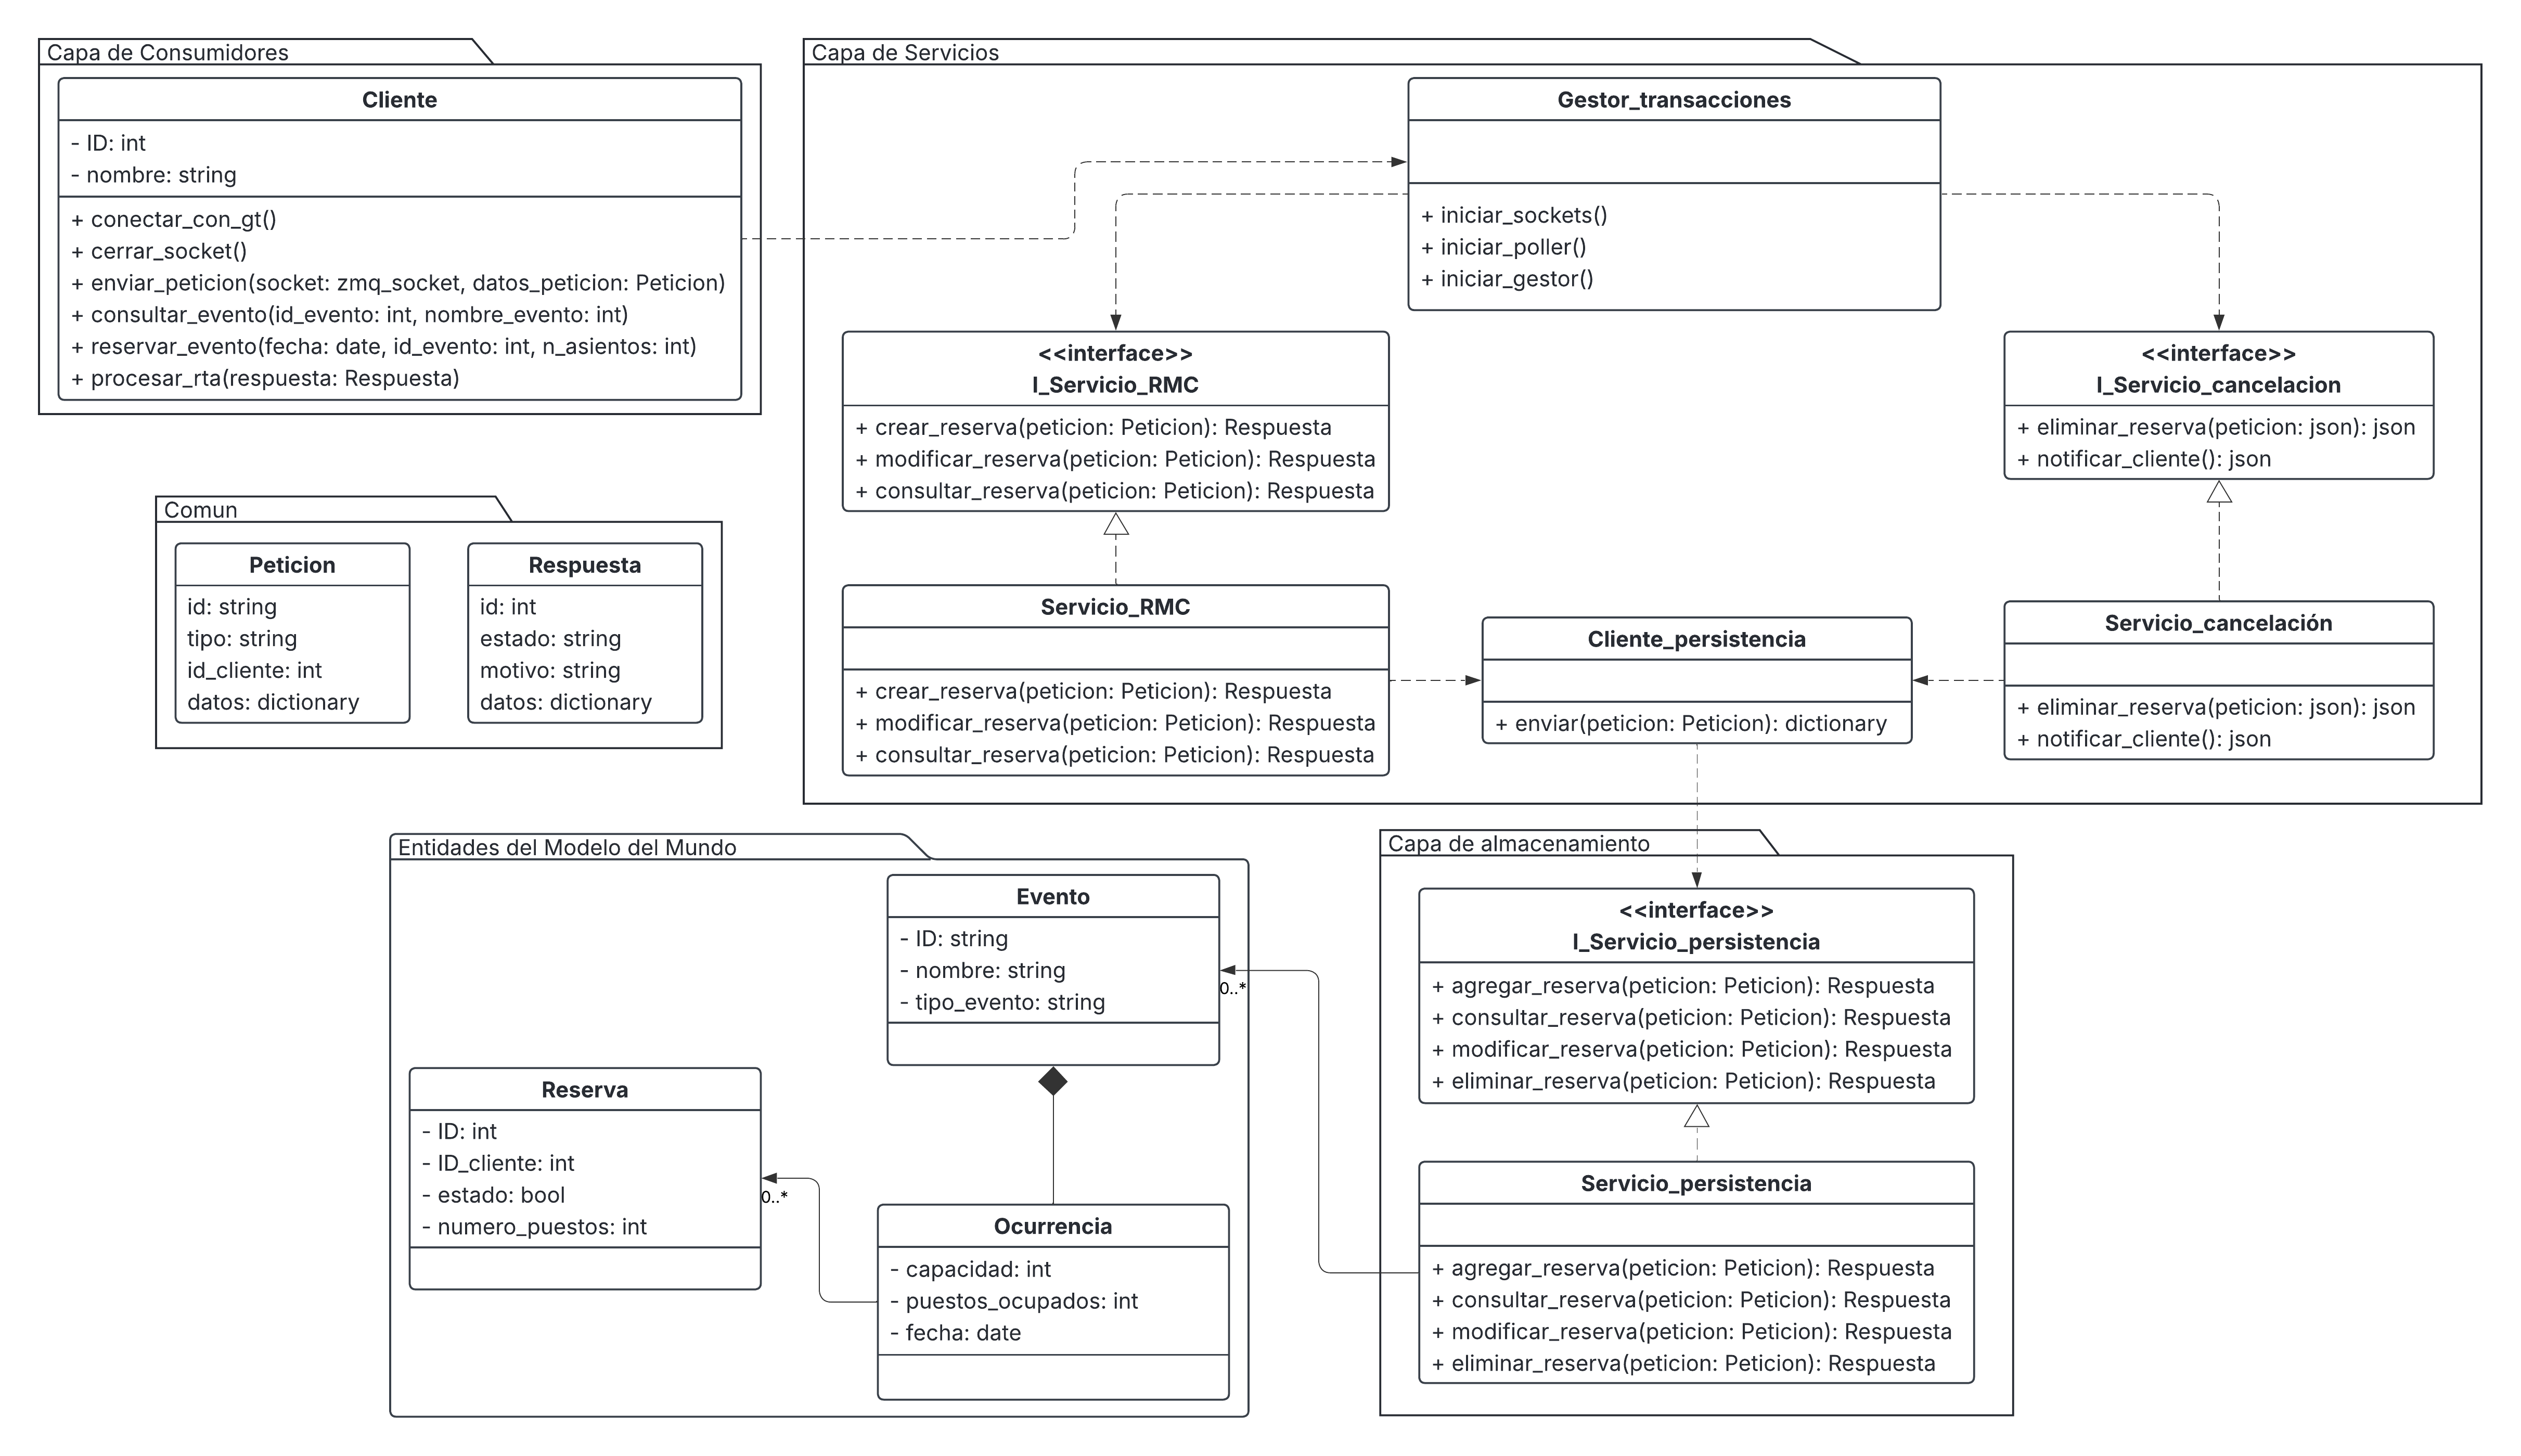
\includegraphics[width=1\textwidth]{Images/Diagrama de Clases.png}
		\caption{Diagrama de clases del SRB}
		\label{fig:class_diagram}
	\end{figure}
	La figura~\ref{fig:class_diagram} muestra las entidades del negocio y las responsabilidades de los servicios. Un Evento tiene identificador, nombre y tipo, y puede tener una o dos Ocurrencias. Cada Ocurrencia tiene su propio identificador, fecha, capacidad y puestos ocupados, de modo que un mismo evento puede repetirse en fechas distintas con disponibilidad independiente. Una Reserva tiene identificador, identificador del cliente, estado y cantidad de puestos, y se asocia a una ocurrencia.

    En la capa de servicios, GestorTransacciones selecciona el canal de atención y mantiene los sockets ROUTER, DEALER y PUSH. ServicioRMC reúne la creación, modificación y consulta de reservas, y ServicioCancelación elimina reservas y notifica al cliente. Ambos usan ClientePersistencia para enviar sus peticiones a ServicioPersistencia, que concentra las operaciones sobre los datos y es el único que habla con la base. Los clientes no acceden a PostgreSQL. La consulta de eventos por mes se detalla en la secuencia siguiente.
	
	\subsection{Diagrama de Secuencia}
	
	\begin{figure}[H]
		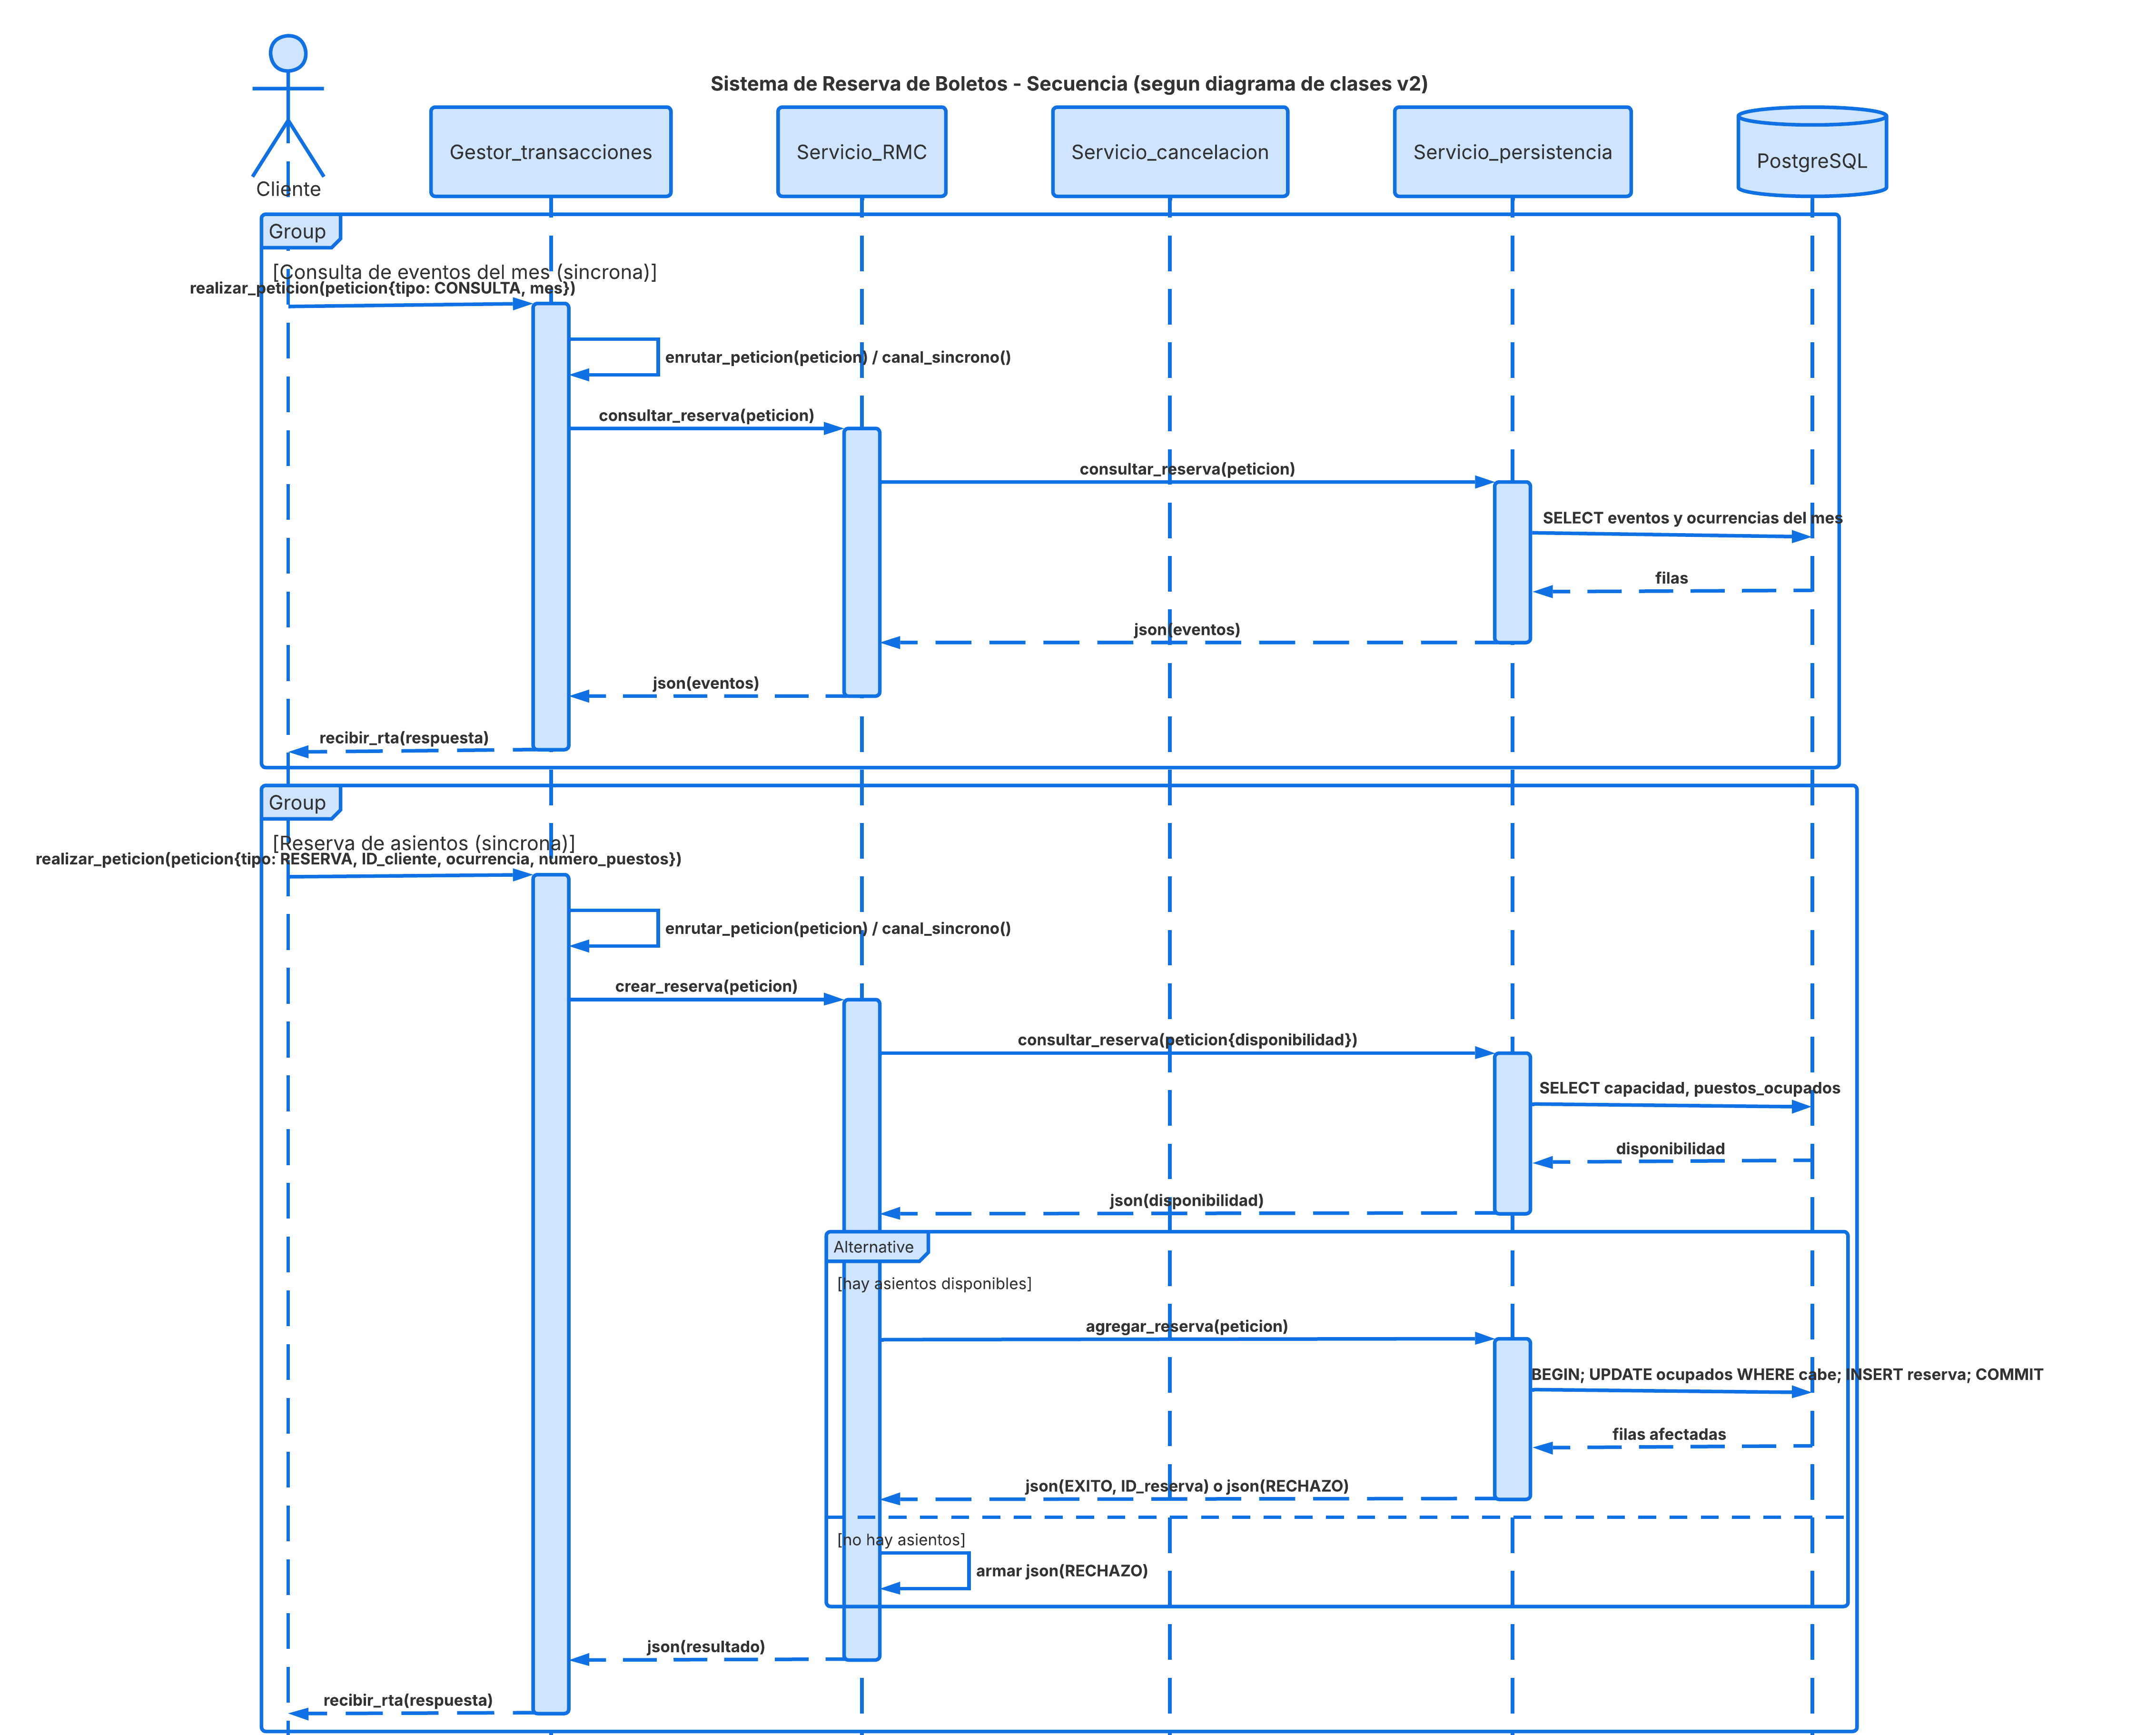
\includegraphics[width=1\textwidth]{Images/Diagrama de Secuencia - 1.png}
		\caption{Secuencia de consulta y reserva del SRB}
		\label{fig:seq_diagram1}
	\end{figure}
	La figura~\ref{fig:seq_diagram1} se lee de arriba hacia abajo y presenta dos operaciones síncronas. En la \textbf{consulta}, el cliente indica el mes al gestor, este remite la petición al RMC y persistencia obtiene los eventos de PostgreSQL. La lista regresa por el mismo recorrido hasta el cliente.

    En la reserva, el cliente envía su identificación, el evento, la fecha de la ocurrencia y la cantidad de puestos. El RMC solicita la disponibilidad y, si existe cupo, pide a persistencia crear la reserva y actualizar la ocupación. El bloque de alternativas distingue la confirmación del rechazo por falta de asientos. La respuesta exitosa, que incluye el identificador de reserva, se devuelve después del COMMIT. Aunque la figura separa la consulta de disponibilidad de la escritura, la implementación deberá volver a comprobar el cupo dentro de la transacción para evitar que solicitudes simultáneas reserven los mismos puestos.
	
	\begin{figure}[H]
		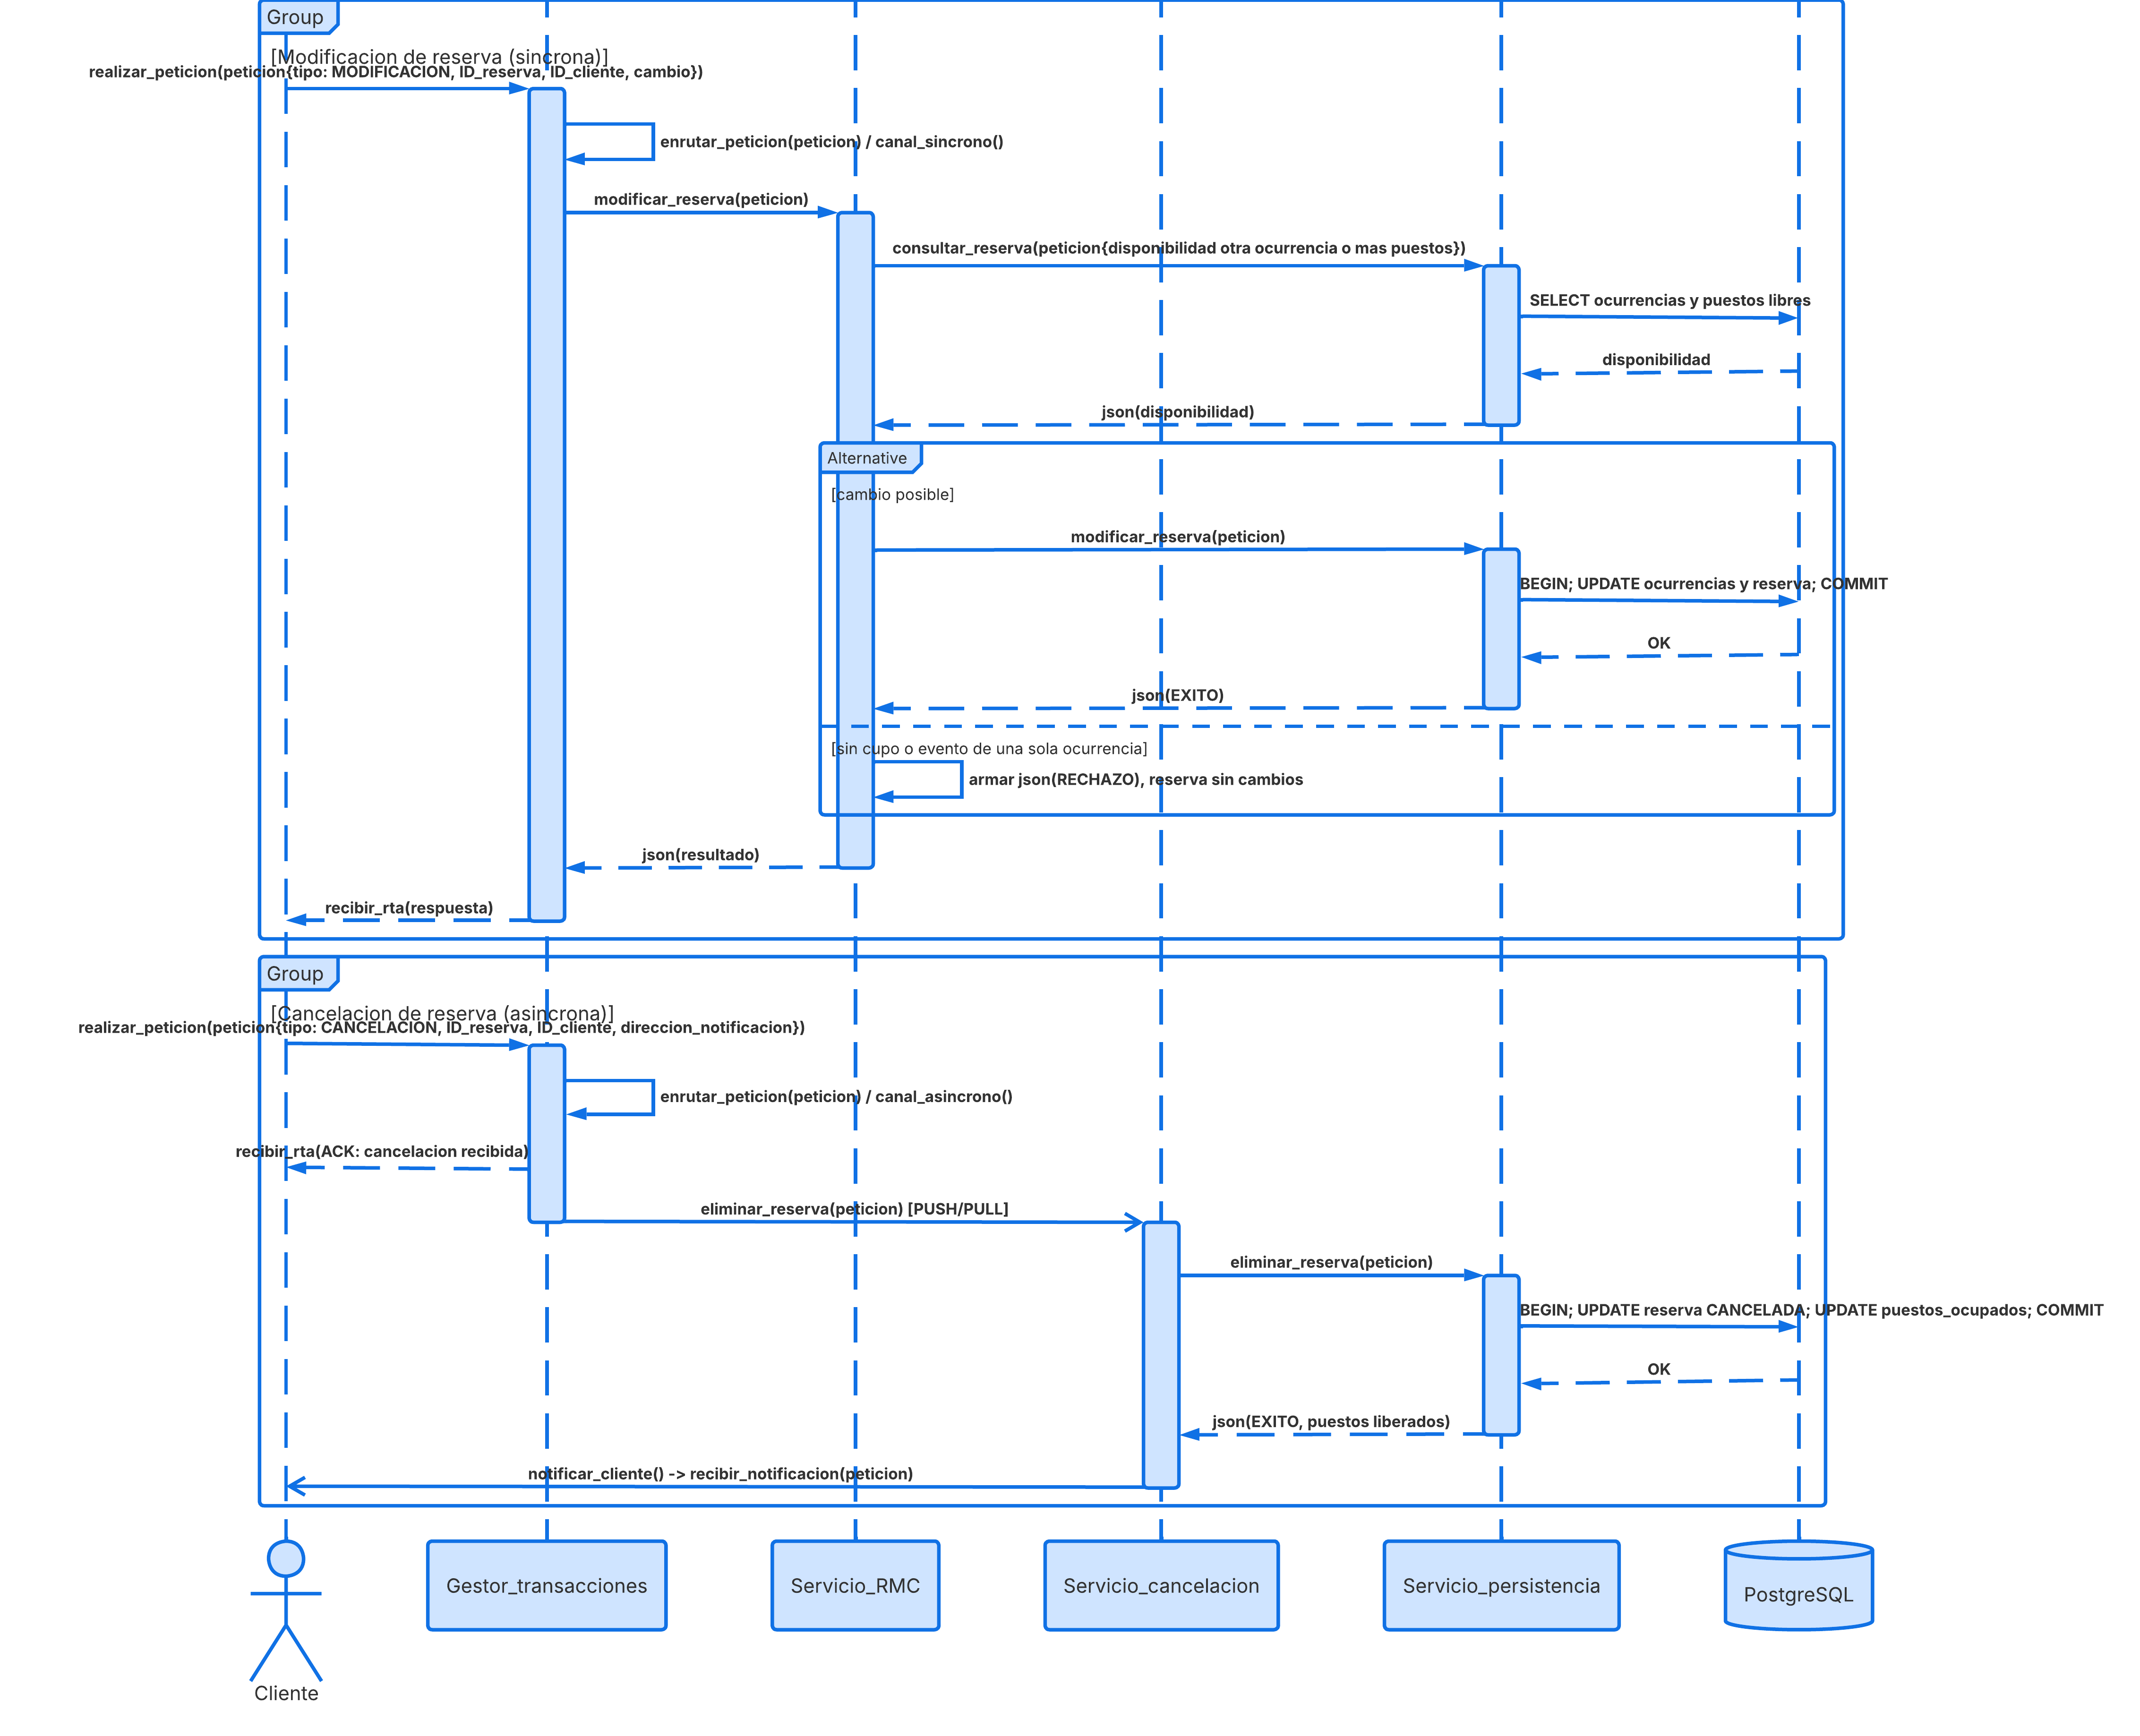
\includegraphics[width=1\textwidth]{Images/Diagrama de Secuencia - 2.png}
		\caption{Secuencia de modificación y cancelación del SRB}
		\label{fig:seq_diagram2}
	\end{figure}
	La figura~\ref{fig:seq_diagram2} continúa con la modificación. El cliente identifica su reserva y el cambio solicitado; el RMC comprueba la disponibilidad mediante persistencia. Si el cambio es válido, se actualizan la reserva y la ocupación en una misma transacción. Si no es posible, se devuelve un rechazo y se conserva la reserva original. El cambio de fecha solo admite otra ocurrencia del mismo evento y mes, manteniendo la cantidad de puestos. Un evento con una sola ocurrencia sí permite modificar esa cantidad, aunque no cambiar de fecha.

    En la cancelación, el cliente incluye la dirección donde recibirá la notificación. El gestor devuelve una aceptación inmediata y envía el trabajo al servicio de cancelación mediante PUSH/PULL. Este solicita a persistencia eliminar la reserva y liberar los asientos. Solo después de confirmar el cambio en PostgreSQL se notifica directamente al cliente. Por tanto, la aceptación inicial indica que la solicitud fue recibida; la notificación posterior confirma que la cancelación se hizo efectiva. El envío final debe dirigirse al receptor de ese cliente, evitando repartir las notificaciones entre clientes distintos.
	
	\section{Estrategia de Escalabilidad y Tolerancia a Fallos}
	\label{sec:scalability}
	La escalabilidad se logra con escalamiento horizontal en la capa que lo necesite. Cada máquina aloja una capa. Los servicios de negocio sin estado, el RMC y el de cancelación, crecen instanciando más réplicas como procesos independientes, que un supervisor lanza y vigila (correr cada proceso en su propio contenedor es una variante de despliegue que no se implementó). El gestor de transacciones reparte el trabajo entre las réplicas del RMC con ROUTER/DEALER y entre las del servicio de cancelación con PUSH/PULL, así que añadir una réplica no exige cambiar el gestor ni los clientes. La capa de persistencia, que sí tiene estado, escala con replicación en streaming de PostgreSQL: un nodo primario atiende las escrituras y las comprobaciones de cupo, y una réplica de solo lectura atiende las consultas de eventos; si la réplica no responde, la consulta se lee del primario. La réplica es asíncrona, de modo que una consulta puede mostrar datos con un retraso de milisegundos, pero ninguna reserva se decide con datos de la réplica, por lo que no puede haber sobreventa. La promoción de la réplica a primario es manual.
	
	Para los fallos \textit{fail-stop} se usan dos mecanismos. Los clientes detectan la falta de respuesta con un \textit{timeout} y reintentan con el mismo identificador de petición; persistencia es idempotente respecto a ese identificador, de modo que una reserva ya confirmada no se duplica. Del lado de los servicios, un supervisor detecta que un proceso terminó (GT, RMC o cancelación) y lanza una copia que lo sustituye; las réplicas se reconectan solas al gestor. No se implementaron señales de vida periódicas: la detección se basa en la terminación del proceso, que es lo que cubre el modelo \textit{fail-stop} adoptado.

	\section{Protocolo de Pruebas de la entrega final}
	\label{sec:protocol}
    Se ejecutarán las siguientes pruebas sobre el sistema final. Cada caso registrará entradas, estado inicial, resultado obtenido y evidencia, para contrastarlos con el resultado esperado.

    \begin{table}[H]
        \centering
        \footnotesize
        \renewcommand{\arraystretch}{1.15}
        \begin{tabular}{@{}p{\dimexpr0.18\linewidth-2\tabcolsep\relax}p{\dimexpr0.42\linewidth-2\tabcolsep\relax}p{\dimexpr0.40\linewidth-2\tabcolsep\relax}@{}}
            \toprule
            \textbf{Tipo de prueba} & \textbf{Procedimiento} & \textbf{Resultado esperado} \\
            \midrule
            Unitarias y límites & Validar meses, cantidades, identificadores y disponibilidad, incluyendo cupo exacto e insuficiente. & Entradas válidas aceptadas; entradas inválidas rechazadas sin cambios en los datos. \\
            Integración & Recorrer el camino cliente, GT, RMC y persistencia, y verificar solicitudes y respuestas. & Respuesta al cliente correcto y confirmación de escritura únicamente después de persistir el cambio. \\
            Funcionales & Consultar, reservar y modificar cantidad o fecha. Probar cambios sin cupo y fechas no permitidas. & Consultas correctas; cambios de fecha dentro del mismo evento y mes, conservando la cantidad. Ante rechazo, reserva original intacta. \\
            Cancelación asíncrona & Solicitar cancelaciones con varios clientes conectados y comprobar las notificaciones. & Aceptación sin esperar la cancelación efectiva; liberación una sola vez y notificación posterior al cliente solicitante. \\
            Concurrencia & Veinte clientes solicitan un asiento cuando quedan diez disponibles. & Diez confirmaciones y diez rechazos, sin sobreventa; libres más ocupados igual a la capacidad. \\
            Fallos y persistencia & Detener GT/RMC antes y después de guardar cambios; sustituir procesos y reintentar con el mismo ID. Reiniciar servicios. & Datos confirmados conservados; continuación de operaciones pendientes sin reiniciar el trabajo del cliente ni duplicar efectos. \\
            Seguridad & Enviar mensajes malformados e intentar modificar o cancelar reservas ajenas. & Rechazo sin cambios no autorizados; el servicio continúa atendiendo solicitudes válidas. \\
            Rendimiento y escalabilidad & Comparar arquitectura base y escalable con el generador de carga propio en los escenarios de 3, 5 y 8 clientes. & Medición de promedio y desviación de latencias de consulta y reserva, y TPM por operación en el GT; comparación mediante tablas y gráficos. \\
            Estrés y duración & Aumentar la carga y mantener una ejecución prolongada. & Identificar saturación, acumulación de pendientes y crecimiento del consumo de recursos. \\
            Despliegue, aceptación y regresión & Ejecutar el README en tres máquinas, aplicar los casos del profesor y repetirlos tras cambios relevantes. & Comunicación entre capas y notificaciones operativas; estado final de la BD acorde con cada caso y funciones previas conservadas. \\
            \bottomrule
        \end{tabular}
        \caption{Protocolo de pruebas previsto para la entrega final.}
        \label{tab:protocol}
    \end{table}

    Las pruebas de rendimiento durarán 2--3 minutos, con al menos 20 solicitudes por minuto por cliente y mezcla parametrizable. En los escenarios de 3, 5 y 8 clientes, respectivamente 2, 3 y 4 solo consultarán; los restantes consultarán y reservarán en el primero, y reservarán y modificarán en los otros dos. Se mantendrán datos iniciales y condiciones equivalentes entre arquitecturas. Se conservarán reportes, logs, estados de la BD y CSV, separando éxitos, rechazos y errores técnicos.
	
	\section{Estrategia de obtención de métricas y carga de los clientes}
	\label{sec:testing}
	% Define the testing protocol for the final delivery.
	% Specify tools/methods for client load generation (Locust or JMeter).
	Para las mediciones se usó un \textbf{generador de carga propio} en Python (\texttt{scripts/benchmark.py}), en lugar de Locust, que era la herramienta prevista inicialmente: cada cliente es un proceso que registra en un CSV el tiempo de cada operación, y de ahí se calculan media, desviación estándar y TPM. Se mantiene la ventaja buscada con Locust (carga desde varios procesos, medición de tiempos y errores), pero sin escribir un adaptador para ZeroMQ.
	
\end{document}
